\documentclass[blue]{beamer}
%\usetheme{Warsaw}
%\usetheme{Boadilla}
%\usetheme{CambridgeUS}
%\usetheme{Berlin}
%\usetheme{Frankfurt}
%\usetheme{Warsaw}
%\usetheme{AnnArbor}
%\usetheme{Antibes}
%\usetheme{Bergen}
%\usetheme{Berkeley}
%\usetheme{Berlin}
%\usetheme{Boadilla}
%\usetheme{boxes}
%\usetheme{CambridgeUS}
%\usetheme{Copenhagen}
%\usetheme{Darmstadt}
%\usetheme{default}
%\usetheme{Dresden}
%\usetheme{Frankfurt}
%\usetheme{Ilmenau}
%\usetheme{Goettingen}
%\usetheme{Hannover}
%\usetheme{JuanLesPins}
%\usetheme{Luebeck}
%\usetheme{Madrid}
%\usetheme{Malmoe}
\usepackage{graphicx}
%\usetheme{Marburg}
%\usetheme{Montpellier}
%\usetheme{PaloAlto}
%\usetheme{Pittsburgh}
%\usetheme{Rochester}
%\usetheme{Singapore}
%\usetheme{Szeged}
\usepackage [autostyle, english = american]{csquotes}
\MakeOuterQuote{"}
%\usecolortheme{dove}
%\usepackage{breqn}

\usepackage[english]{babel}
\usepackage[latin1]{inputenc}
\usepackage{bbm}
\setbeamercovered{transparent}

\title{Lecture in Labour Economics}
\subtitle{ }
\author[Karimzada]{Muhebullah Karimzada}
\institute{\textit{McMaster University}}
%\institute{Future of Growth Conference}
\bigskip
\date[ ]{July 02, 2024}
%\date[ 

\begin{document}
\frame{\titlepage}
\label{Learning Objectives}
\begin{frame} \frametitle{Learning Objectives}

 		 	\begin{enumerate}
 		 
 		\item 	Using the labour supply model, analyse the work incentive effects of the following policies:
 		
 		\begin{enumerate}[a]
 		 \item []
 		\item Unemployment insurance benefits
 		
 		 \item Child care benefit
 		\end{enumerate}
 		   \item []
 		   \item Explain how imperfect information can lead to a labour market equilibrium in which unemployed workers and unfilled job vacancies co-exist
         \end{enumerate}
        
      %
\end{frame}



\begin{frame} \frametitle{Unemployment Insurance Benefits}
\label{Unemployment Insurance Benefits}

\begin{itemize}
\item Canada's unemployment insurance program, known as Employment Insurance EI since 1996, is the largest income security program for non-elderly individuals in the country
\item[]
\item The amount of income replacement rate is $55\%$ of lost earning, subject to a maximum
\item[]
\item The duration of benefit ranges from 14 to 45 weeks, depending on the regional rate of unemployment
\item[]
 \item In order to qualify for the benefits, individuals must have worked between 420 and 700 hours, the equivalent of 12-20 weeks at 35 hours per week, again depending on the unemployment rate of the region.
 \end{itemize}
 \end{frame}


\begin{frame} \frametitle{Unemployment Insurance Benefits}
\label{Unemployment Insurance Benefits}

Example\\

Analysing the work incentive effects of unemployment insurance using the income-leisure model of the labour supply 

\begin{itemize}
\item[]
\item Recipients receive 60 percent of their weekly pay in the case of unemployment 

\item[]
\item It requires a minimum of 14 weeks of employment in order to qualify for benefits.

\item[]
\item The maximum period of receiving benefits is 20 weeks
\item[]
\item For simplicity,  we use one-year time horizon
 \end{itemize}
 \end{frame}
 
 
 
 \begin{frame}
  \frametitle{Income Constraint for a Simplified Unemployment Insurance Scheme
}
\begin{figure}
    \begin{center}
      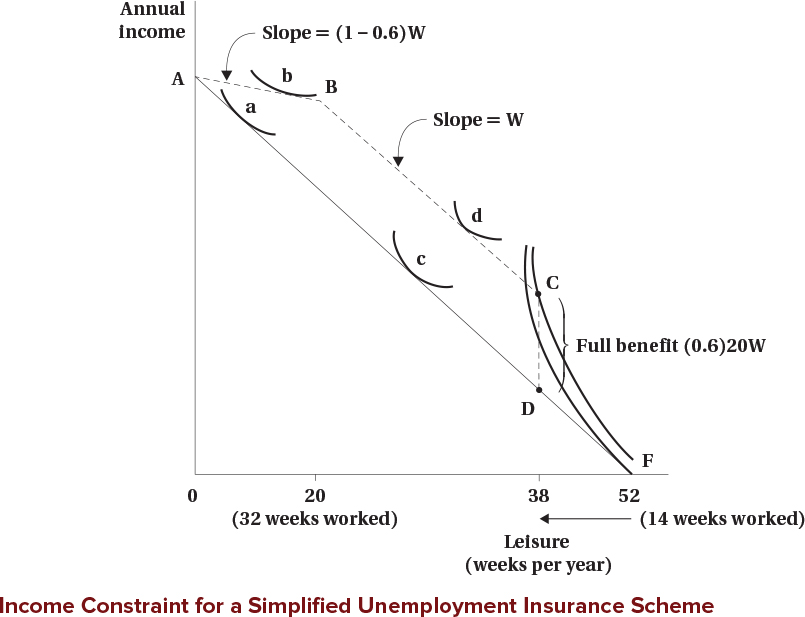
\includegraphics[scale=0.7923]{EI.jpg}
      %    \includegraphics[scale=.40]{one.pdf}
      \end{center}
  \end{figure}
\end{frame}
 
 
 \begin{frame} \frametitle{Income Constraint for a Simplified Unemployment Insurance Scheme}


\begin{itemize}
\item[]
\item AF (solid line)- potential income constraint in the absence of unemployment insurance (UI) program

\item[]
\item ABCDF- constraint with UI

\item[]
\item If the individual works less than 14 weeks during the year,  they do not qualify for UI benefits - their income constraint is segment DF
\item[]
\item If the individual works 14 weeks,  they are eligible for benefits for an additional 20 weeks
\item[]
\item Their income at 14 weeks of work equals their labour market earning for the 14 weeks plus 20 times 60 percent of their normal weekly wage earnings
\item[]
\item Their annual income would be $Y=14W +(0.60)20W$
 \end{itemize}
 \end{frame}
 
 
 
 \begin{frame} \frametitle{Income Constraint for a Simplified Unemployment Insurance Scheme}


\begin{itemize}
\item[]
\item Their annual income would be $Y=14W +(0.60)20W$
\begin{itemize}
\item W is weekly wage earnings
\item $(0.60)20W$ - full benefit (vertical distance between C and D)
\item[]
\end{itemize}
 \end{itemize}

The work incentive effects of UI depend on where the individual would be located in the absence of UI system - three different possibilities

\begin{enumerate}
\item Individuals working more than 32 weeks (e.g. point a on AF)

\begin{itemize}
\item The income and substitution effects work in the same direction to potentially decrease weeks worked (moving to point b on AB)
\end{itemize}

\item Individuals such as those originally at point c on AF
\begin{itemize}
\item the UI system constitutes pure income effect - potentially decreasing work incentives (moving to point d on AB)
\end{itemize}
\end{enumerate}
 \end{frame}
 
 
  \begin{frame} \frametitle{Income Constraint for a Simplified Unemployment Insurance Scheme}




\begin{enumerate}
\setcounter{enumi}{2}
\item Individuals who would be outside the labour force in the absence of UI program
\begin{itemize}
\item[]
\item originally locted at point F -  reflecting the high value of their time devoted to non-market activities
\item[]
\item many of these individuals neither work nor collect UI
\item[]
\item others would enter the labour force and work a sufficient number of weeks to qualify for UI benefits (point C)
\begin{itemize}
\item[]
\item UI program has increased work incentives by making it attractive for these individuals to devote less time to non-market activities and to enter the labour force for relatively brief periods.
\end{itemize}
\end{itemize}
\end{enumerate}
 \end{frame}
 
 
 
 
 
 
 
 
 \begin{frame} \frametitle{Child Care Benefit}
\label{Child Care Benefit}

\begin{itemize}
\item Analysis of the child care benefit first requires an investigation of how child care costs might affect a parent's labour supply decision

\item Child care costs can be modelled as a special case of fixed costs associated with working

\item Assumptions:
\begin{itemize}


 \item child care cost is incurred only if the person works in paid labour market
\item child care cost is independent of hours worked
\item[]
\end{itemize}

 \end{itemize}
 \end{frame}
 
 
  \begin{frame}
  \frametitle{The effect of Child Care Costs on Labour Supply
}
\begin{figure}
    \begin{center}
      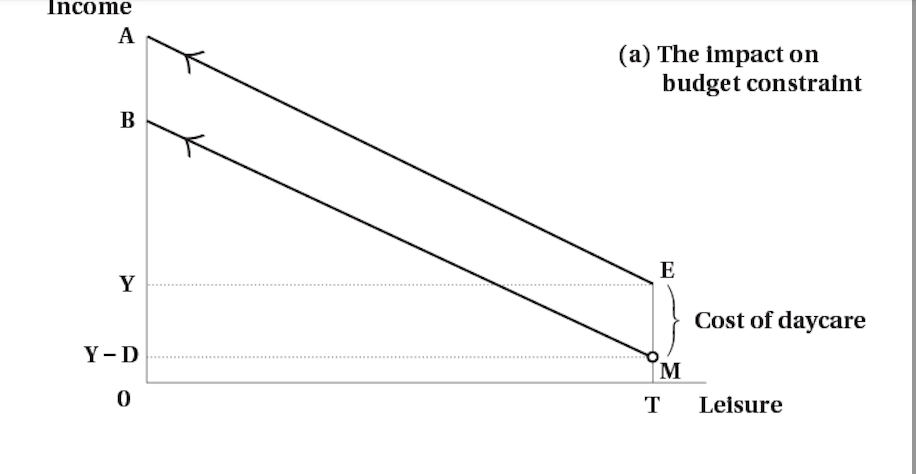
\includegraphics[scale=0.76]{CCB1.png}
      %    \includegraphics[scale=.40]{one.pdf}
      \end{center}
  \end{figure}
\end{frame}
 
 
   \begin{frame}
  \frametitle{The effect of Child Care Costs on Labour Supply}
The impact on budget constraint:

\begin{itemize}

\item the fixed cost of child care is analogous to a vertical drop in the individual's budget constraint immediately upon entering the labour market
\begin{itemize}
\item[]
\item the individual incurs the fixed costs D=EM $\rightarrow$ analogous to a drop in income of EM
\item[]
\item point M is slightly to the left of the vertical line ET - indicating that costs are incurred only if one engages in labour market activity
\item[]
\item fixed costs are avoided if one does not work in the labour market but remains at E

\end{itemize}
\end{itemize}
Summary:
\begin{itemize}
\item Income constraint AE - in the absence of child care costs
\item Income constraint BME - with fixed child care costs
\end{itemize}
\end{frame}
 
 
 %   \begin{frame}
 % \frametitle{The effect of Child Care Costs on Labour Supply
%}
%\begin{figure}
  %  \begin{center}
   %   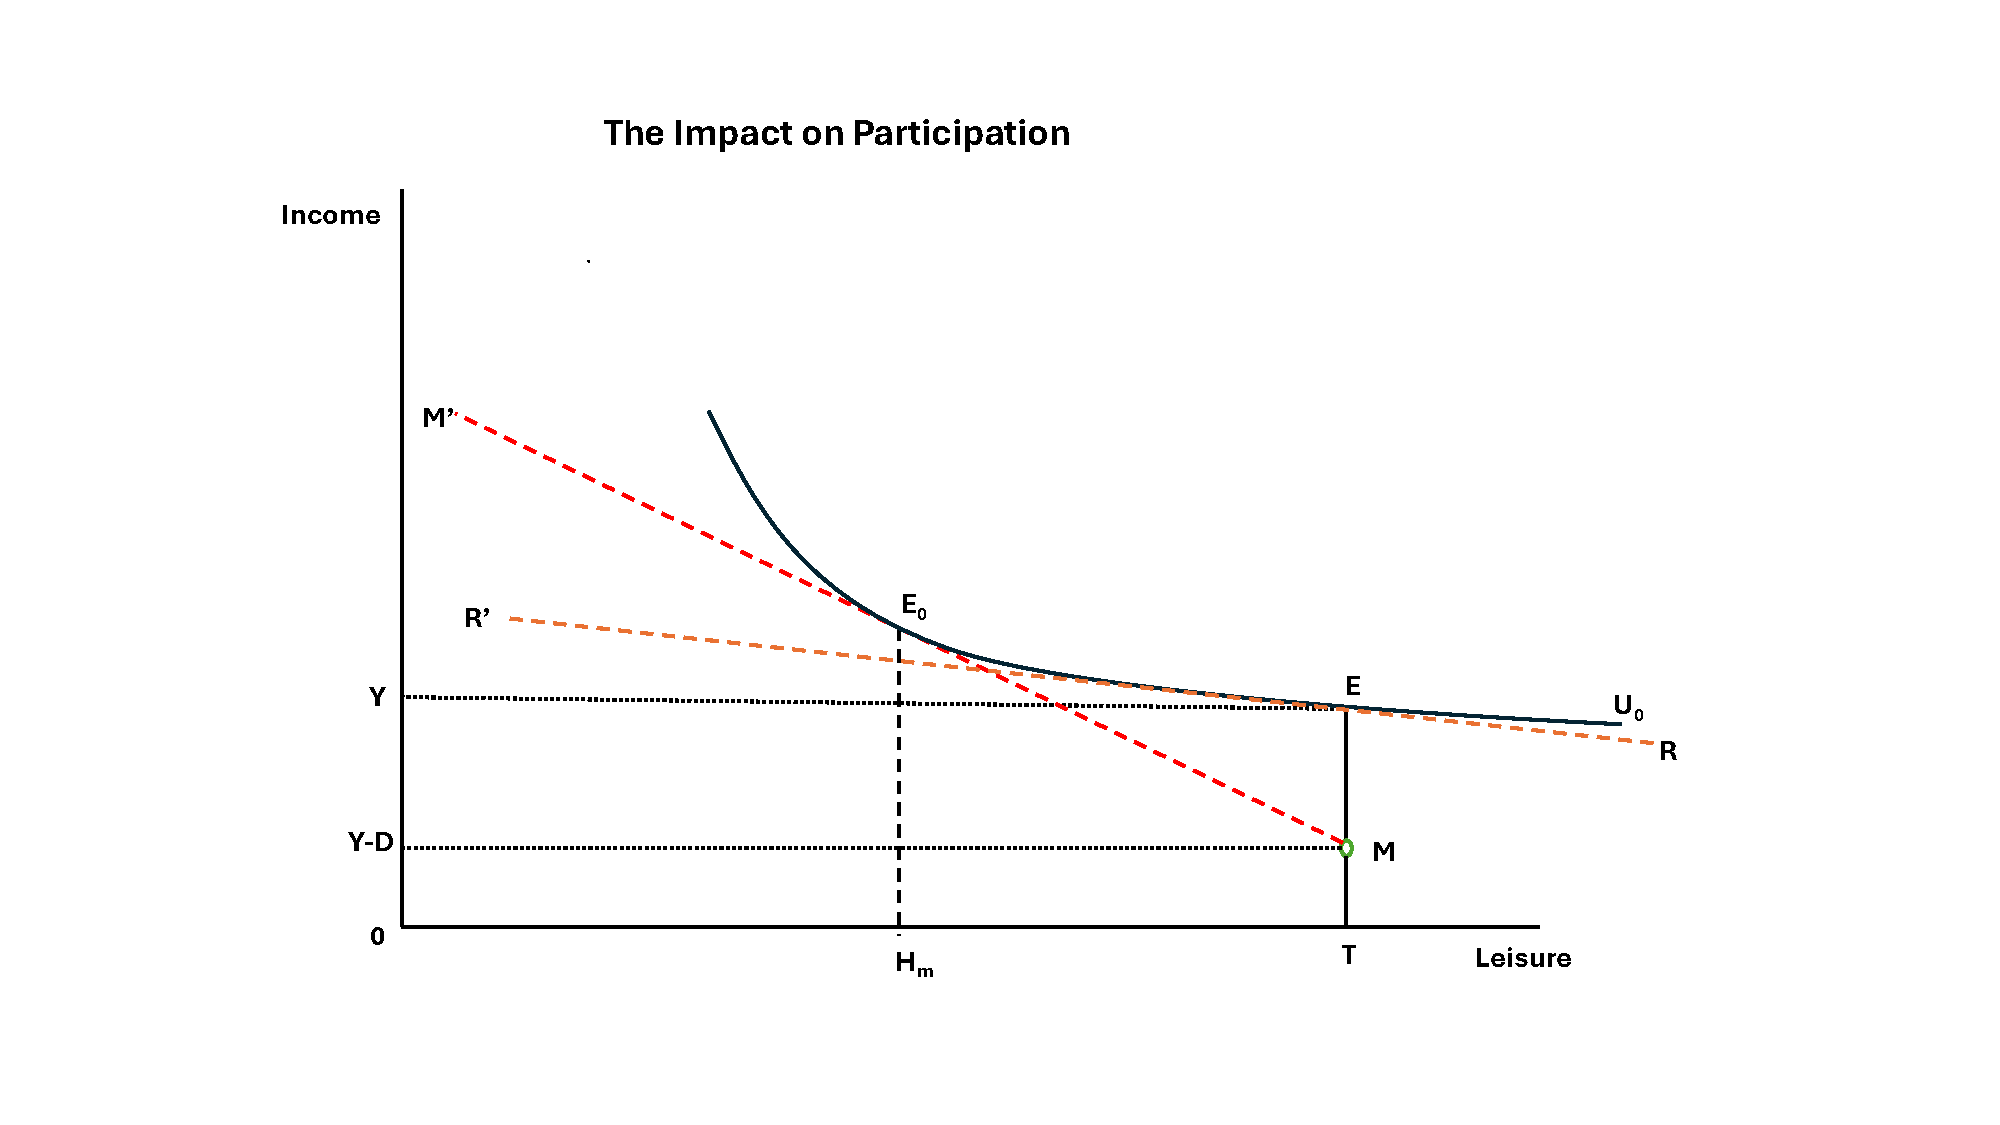
\includegraphics[scale=0.4]{Presentation1b.pdf}
      %    \includegraphics[scale=.40]{one.pdf}
   %   \end{center}
 % \end{figure}
%\end{frame}

   \begin{frame}
  \frametitle{The effect of Child Care Costs on Labour Supply
}
\begin{figure}
    \begin{center}
      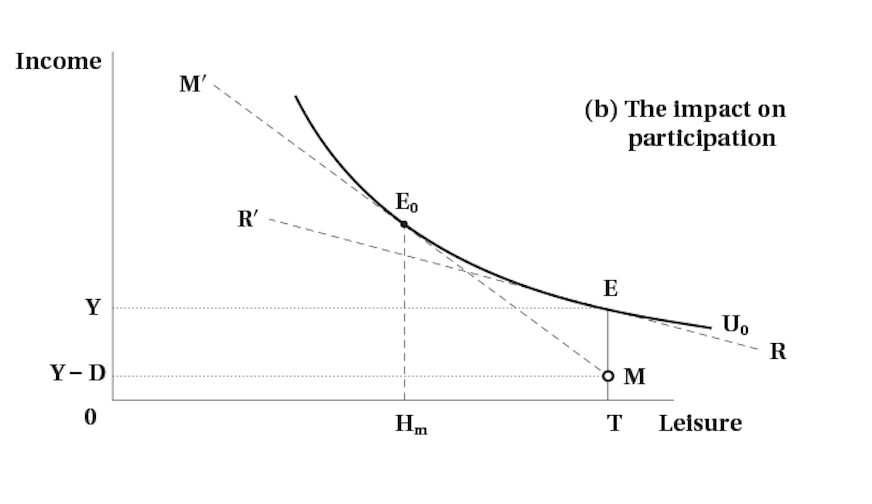
\includegraphics[scale=0.76]{CCB2.png}
      %    \includegraphics[scale=.40]{one.pdf}
      \end{center}
  \end{figure}
\end{frame}
 
 
   \begin{frame}
  \frametitle{The effect of Child Care Costs on Labour Supply}
The impact on participation:

\begin{itemize}
\item In the absence of child care fixed costs, the individual's reservation wage is depicted by the slope RR'
\item[]
\item In the presence of child care fixed costs, the individual's reservation wage is depicted by the slope MM'
\begin{itemize}
\item[]
\item the minimum wage above which one would enter the labour market
\item[]
\item at this wage one would be indifferent between engaging in labour market activities at $E_{0}$ and remaining at home with children at E
\item[]
\end{itemize}

\item Market wage greater than the reservation wage would induce labour force participation and the amount of work would be determined by the tangency of new, higher indifference curve and a higher budget constraint

\end{itemize}

\end{frame} 
 
 
    \begin{frame}
  \frametitle{The effect of Child Care Costs on Labour Supply}
The impact on participation:

\begin{itemize}

\item the line MM' is tangent to $U_{0}$ at the point  $E_{0}$ that is to the left of E of the same indifference curve
\item[]
\item the indifference curve become steeper as one moves to the left of E because of the hypothesis of diminishing marginal rate of substitution
\item[]
\item child care costs associated with entering the labour market increase the reservation wage by making labour market work less attractive than caring for the children at home

\end{itemize}

\end{frame} 
 
 
    \begin{frame}
  \frametitle{The effect of Child Care Costs on Labour Supply
}
\begin{figure}
    \begin{center}
      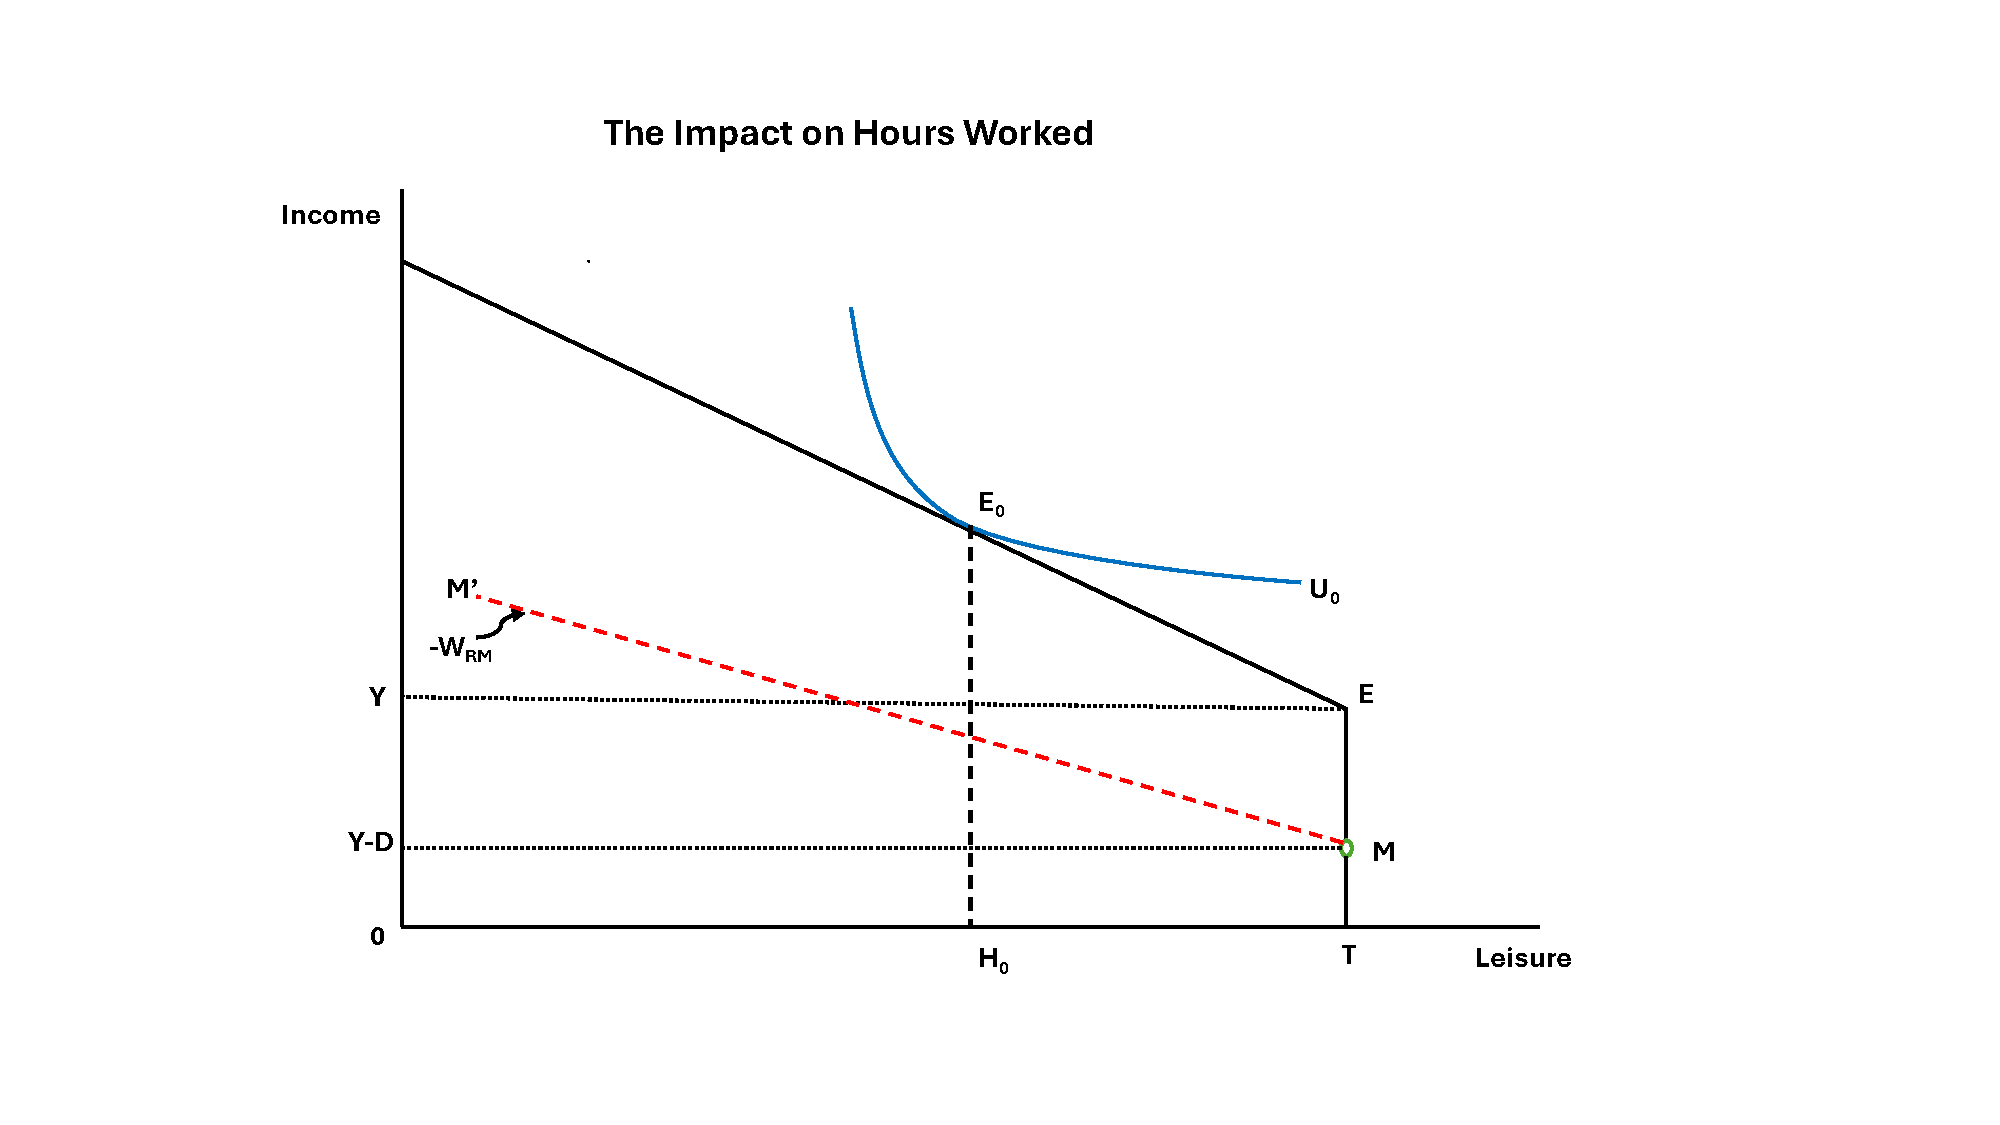
\includegraphics[scale=0.43]{Presentation2.pdf}
      %    \includegraphics[scale=.40]{one.pdf}
      \end{center}
  \end{figure}
\end{frame}
 
    \begin{frame}
  \frametitle{The effect of Child Care Costs on Labour Supply
}
\begin{figure}
    \begin{center}
      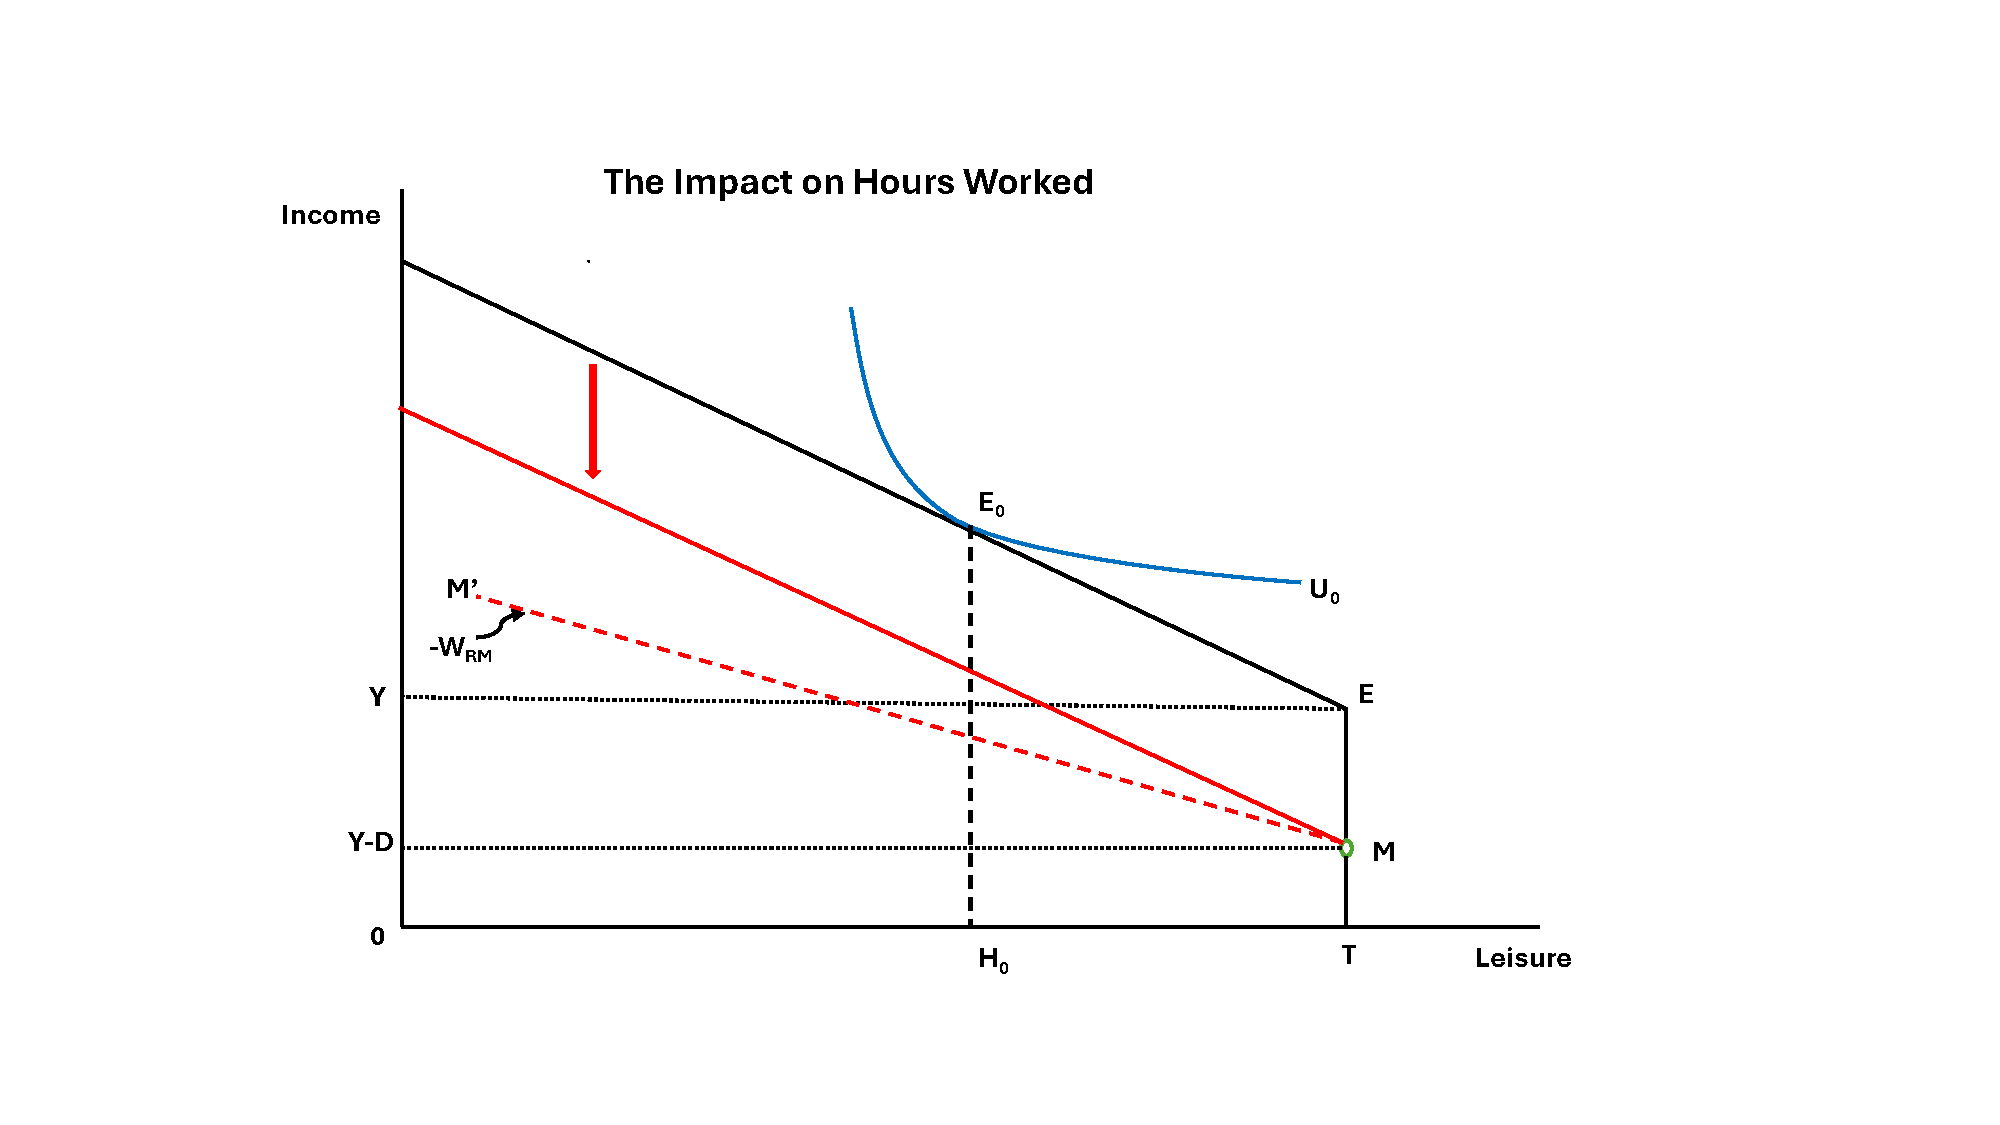
\includegraphics[scale=0.43]{Presentation3.pdf}
      %    \includegraphics[scale=.40]{one.pdf}
      \end{center}
  \end{figure}
\end{frame}

    \begin{frame}
  \frametitle{The effect of Child Care Costs on Labour Supply
}
\begin{figure}
    \begin{center}
      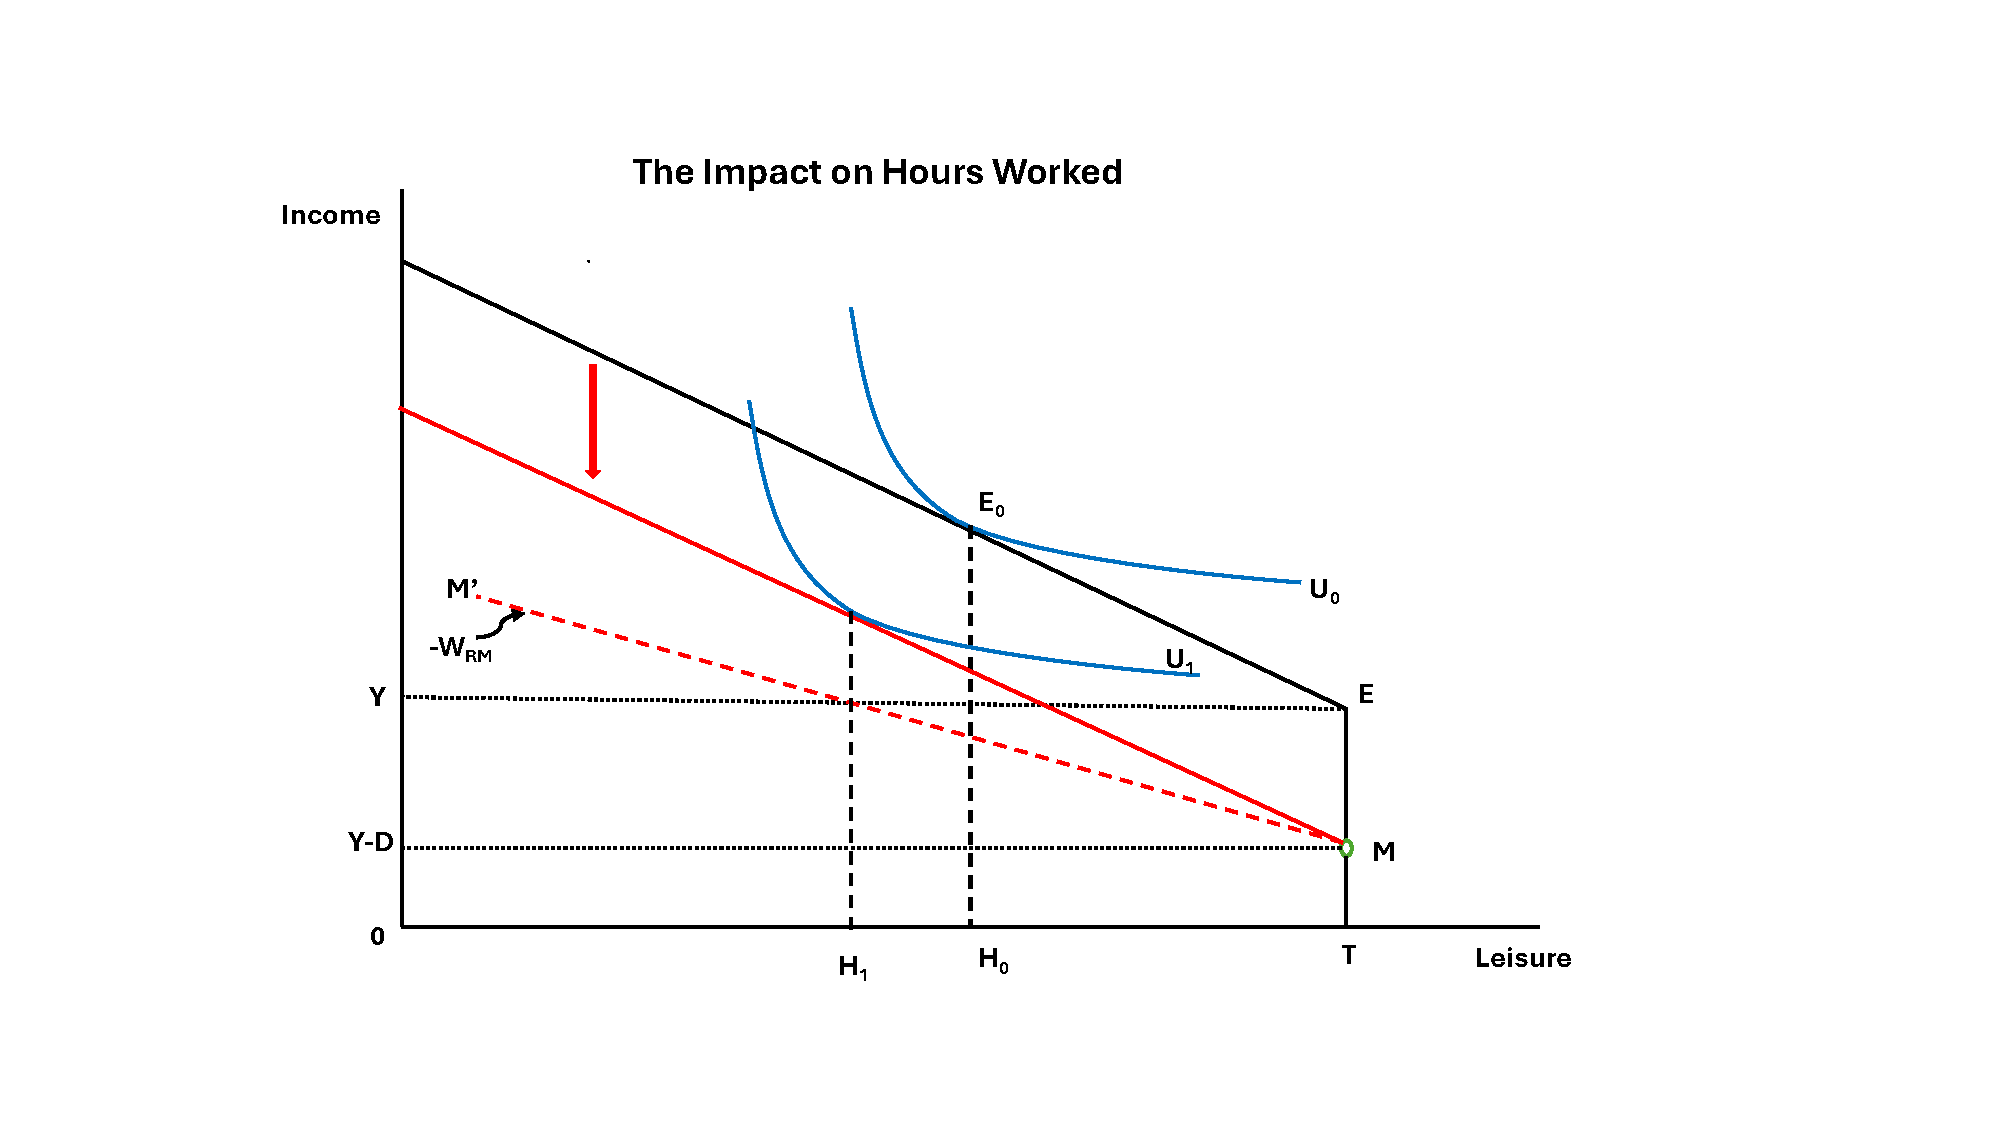
\includegraphics[scale=0.43]{Presentation4.pdf}
      %    \includegraphics[scale=.40]{one.pdf}
      \end{center}
  \end{figure}
\end{frame}

    \begin{frame}
  \frametitle{The effect of Child Care Costs on Labour Supply
}
\begin{figure}
    \begin{center}
      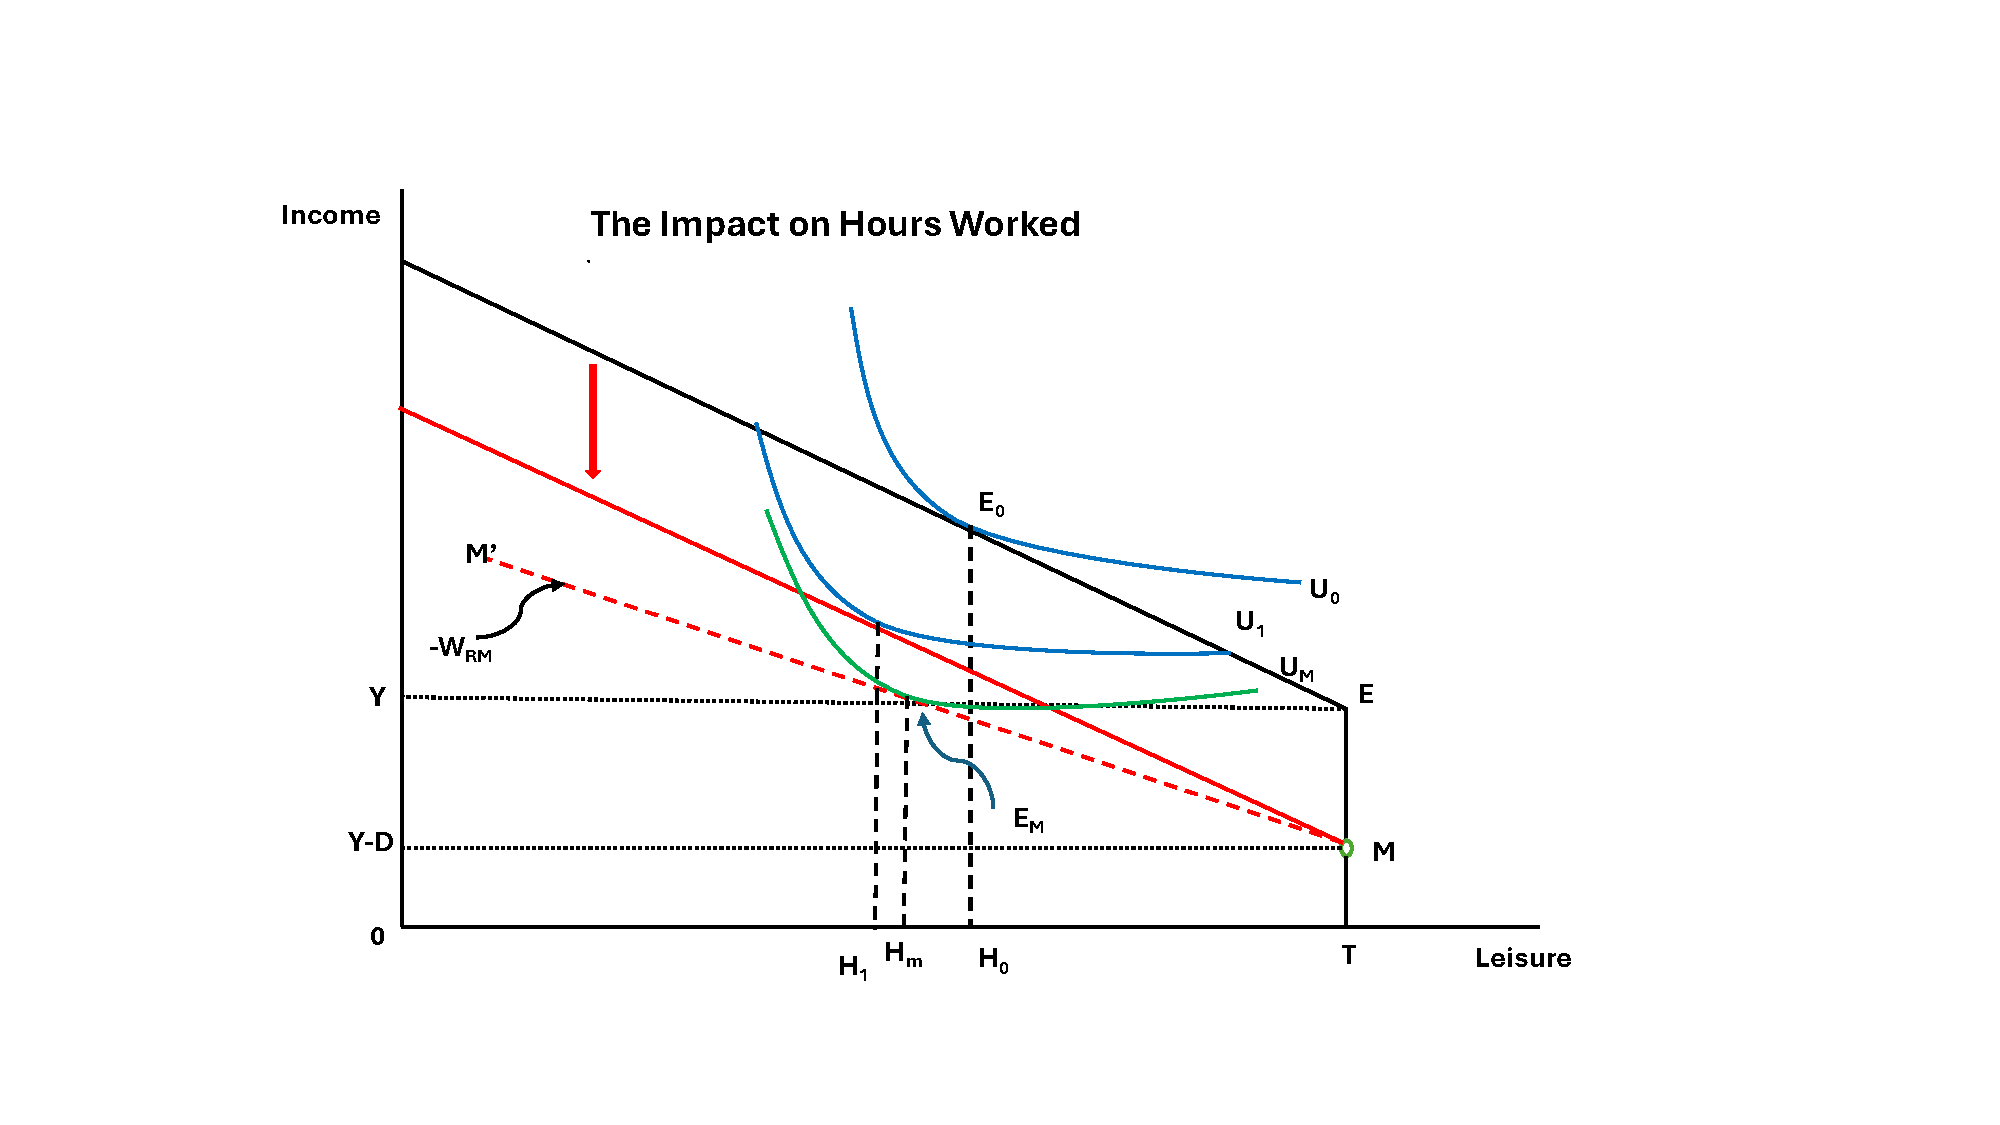
\includegraphics[scale=0.43]{Presentation5.pdf}
      %    \includegraphics[scale=.40]{one.pdf}
      \end{center}
  \end{figure}
\end{frame} 
 
 
 
 
 
 
   \begin{frame}
  \frametitle{The effect of Child Care Costs on Labour Supply
}
\begin{figure}
    \begin{center}
      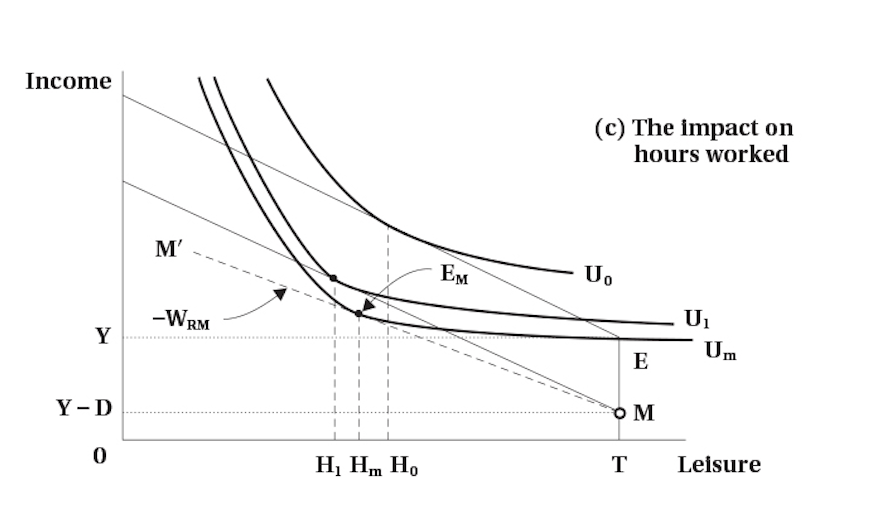
\includegraphics[scale=0.76]{CCB3.png}
      %    \includegraphics[scale=.40]{one.pdf}
      \end{center}
  \end{figure}
\end{frame}
 
 
    \begin{frame}
  \frametitle{The effect of Child Care Costs on Labour Supply}
\textbf{The impact on hours worked:}

\begin{itemize}

\item initial equilibrium:  at $E_{0}$ with hours of work $H_{0}$  and no child care costs
\item[]
\item the existence of fixed child care costs shifts the budget constraint down in a parallel fashion because market wages have not changed

\item[]
\item if leisure is a normal good - this pure income effect from the reduced income increases hours of work from $H_{0}$ to $H_{1}$ 
\item[]
\item when there are fixed costs, one has to work more hours to make up for the income loss associated with the costs of child care.

\end{itemize}

\end{frame}  
 
 
     \begin{frame}
  \frametitle{The effect of Child Care Costs on Labour Supply}



\textbf{Fixed child care costs also create a discontinuity or gap in the implied labour supply schedule}

\begin{itemize}
\item[]
\item the distance $TH_{m}$ indicates the number of hours below which it would not be worthwhile to enter the labour market - given the reservation wage $W_{RM}$ created by the child care costs EM

\item[]
\item it is not possible to amortize the fixed costs of entering the labour force over so few hours $\rightarrow$ there is a discrete jump in the labour supply from zero to $TH_{m}$ 
\item[]
\item geometrically,  it is not possible for there to be a tangency between the budget constraint MM' and the indifference curve $U_{M}$ in the region $E_{M}E$

\begin{itemize}
\item the slope of MM' is always greater than the slope of the indifference curve to the right $E_{M}$
\item in this way,  the child care costs discourage part-time work
\end{itemize}

\end{itemize}

\end{frame}  
 
 
 
  \begin{frame} \frametitle{Child Care Benefit}
\label{Child Care Benefit}

\begin{itemize}


\item Effects of child care costs

\begin{itemize}
\item Fixed child care costs increase reservation wage - decrease labour force participation

\item Fixed child care costs also affect hours-of-work
\begin{itemize}
\item Increased hours for those who participate
\item Create a discontinuity in labour supply -  making part-time work less likely
\item[]
\end{itemize}
\end{itemize}
\end{itemize}

Therefore,  child care benefit:
\begin{itemize}
\item encourages labour force participation and part-time work
\item[]
\item reduces the hours of work for those already participating
 \end{itemize}
 \end{frame}
 
 
 
 
   \begin{frame} \frametitle{Imperfect Information in the Labour Market}
\label{imperfect info and labour market}

\begin{itemize}
\item Imperfect information in the labour market can result in a situation where both job vacancies and unemployed workers exist simultaneously
\item[]
\item frictional unemployment - unemployment associated with normal turnover in the labour market
\item[]
\item structural unemployment -mismatch between labour demand and labour supply,  either on occupational,  skills, or regional dimensions


 \end{itemize}
 \end{frame}
 

   \begin{frame} \frametitle{Imperfect Information in the Labour Market}
\label{imperfect info and labour market}

\begin{itemize}

\item the job search and matching process is associated with imperfect information on both sides of the labour market

\item unemployed workers are not aware of 
\begin{itemize}
\item all available jobs 
\item their rates of pay
\item location
\item working condition
\end{itemize}
\item[]
\item employers with job vacancies are not aware of all individual workers and their characteristics
\item[]
\item if both sides were fully informed, the process of matching workers and jobs could take place in a few days, if not hours. 
\item[]
\item since the acquisition of information about job opportunities and job applicants takes time, unemployment and vacancies co-exist.
 \end{itemize}
 \end{frame}



   \begin{frame} \frametitle{Imperfect Information in the Labour Market}
\label{imperfect info and labour market}

\begin{itemize}

\item Job search is an economic decision in that it involves both costs and benefits
\item two main aspects to the decison:
\begin{itemize}
\item determining whether it is worthwhile initiating the job search process
\item determining when to stop the process
\end{itemize}
\item Expected benefits have to be weighted against the expected costs
\item Employees continue to search until expected marginal benefit equal expected marginal cost
\item Benefits and costs of search are likely to be related to the amount of time devoted to a job search
\item Marginal cost is rising with the amount of job search undertaken

 \end{itemize}
 \end{frame}

   \begin{frame}
  \frametitle{Optimal Job Search}
\begin{figure}
    \begin{center}
      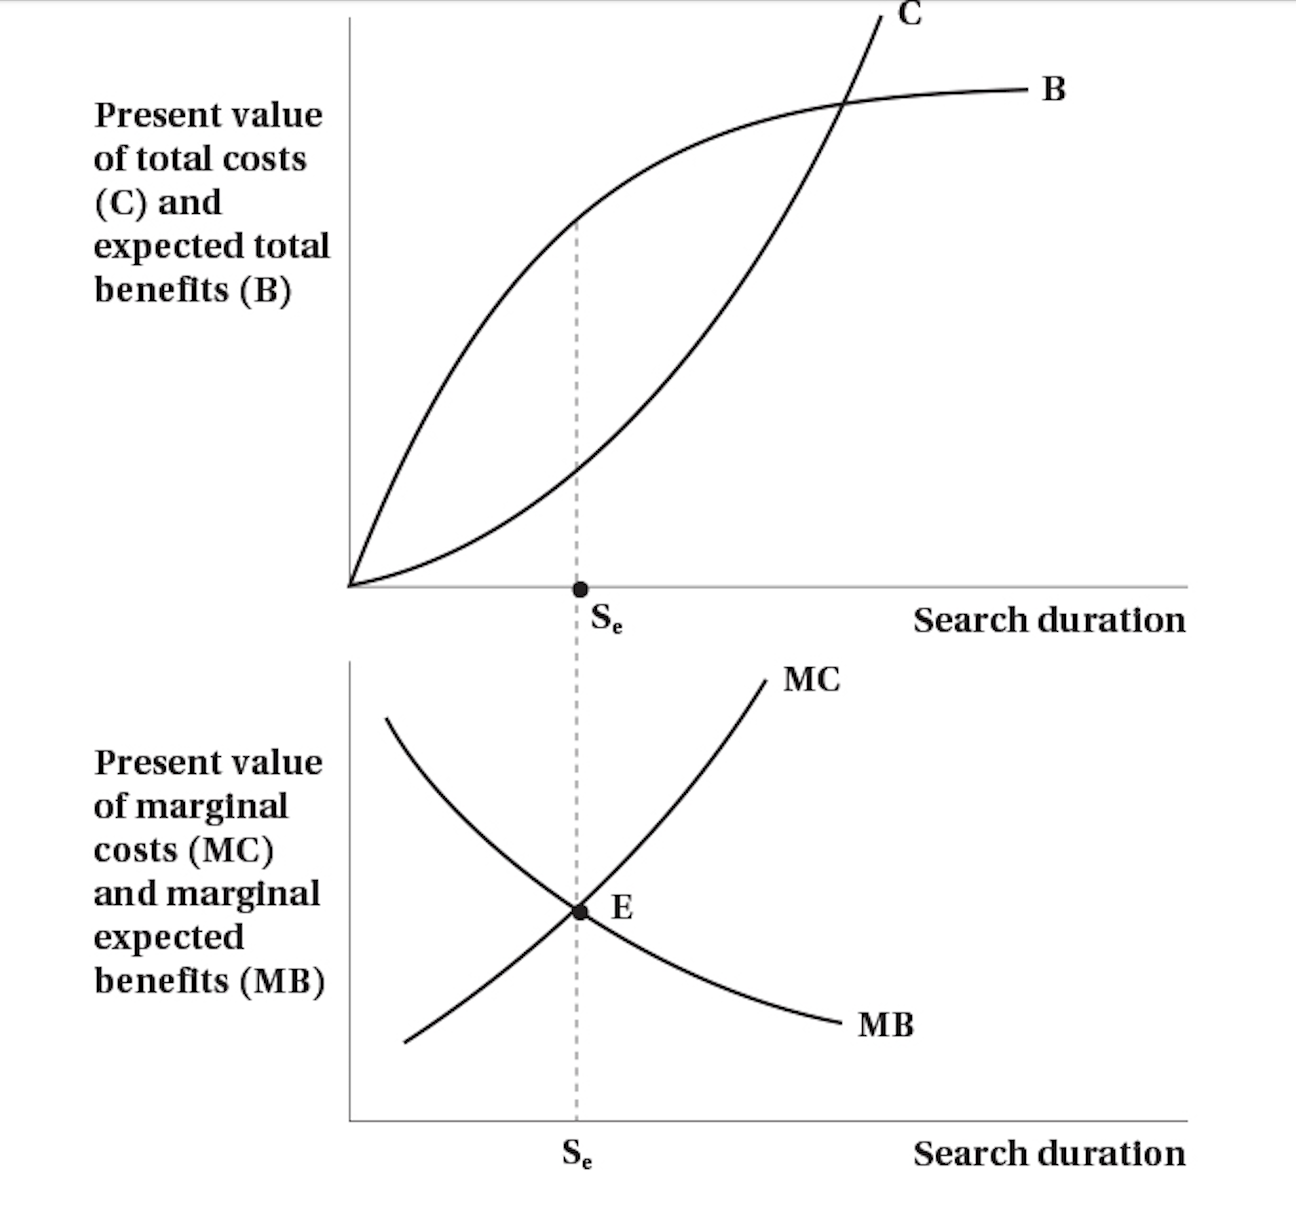
\includegraphics[scale=0.4]{MC_MB.png}
      %    \includegraphics[scale=.40]{one.pdf}
      \end{center}
  \end{figure}
\end{frame}



   \begin{frame} \frametitle{Imperfect Information in the Labour Market}
\label{imperfect info and labour market}

\begin{itemize}

\item Optimal amount of a search will maximize the difference between B and C 

\item The difference is maximized when expected marginal  benefit equals expected marginal cost at Se 
 \end{itemize}
 \end{frame}


  \begin{frame} \frametitle{Imperfect Information in the Labour Market}
\label{imperfect info and labour market}


\textbf{Implications of imperfect information}

Generally workers and firms will stop their search activities prior to being fully informed due to diminishing returns to information acquisition and also increasing costs of information acquisition. As a result:
\begin{itemize}
\item A labour market characterized by imperfect information will not clear instantaneously
\item Dispersion of wage rates will occur even in a labour market with homogeneous workers and jobs
\end{itemize}

 \end{frame}


  \begin{frame}
  \frametitle{Wage Distribution Under Imperfect and Perfect Information}
\begin{figure}
    \begin{center}
      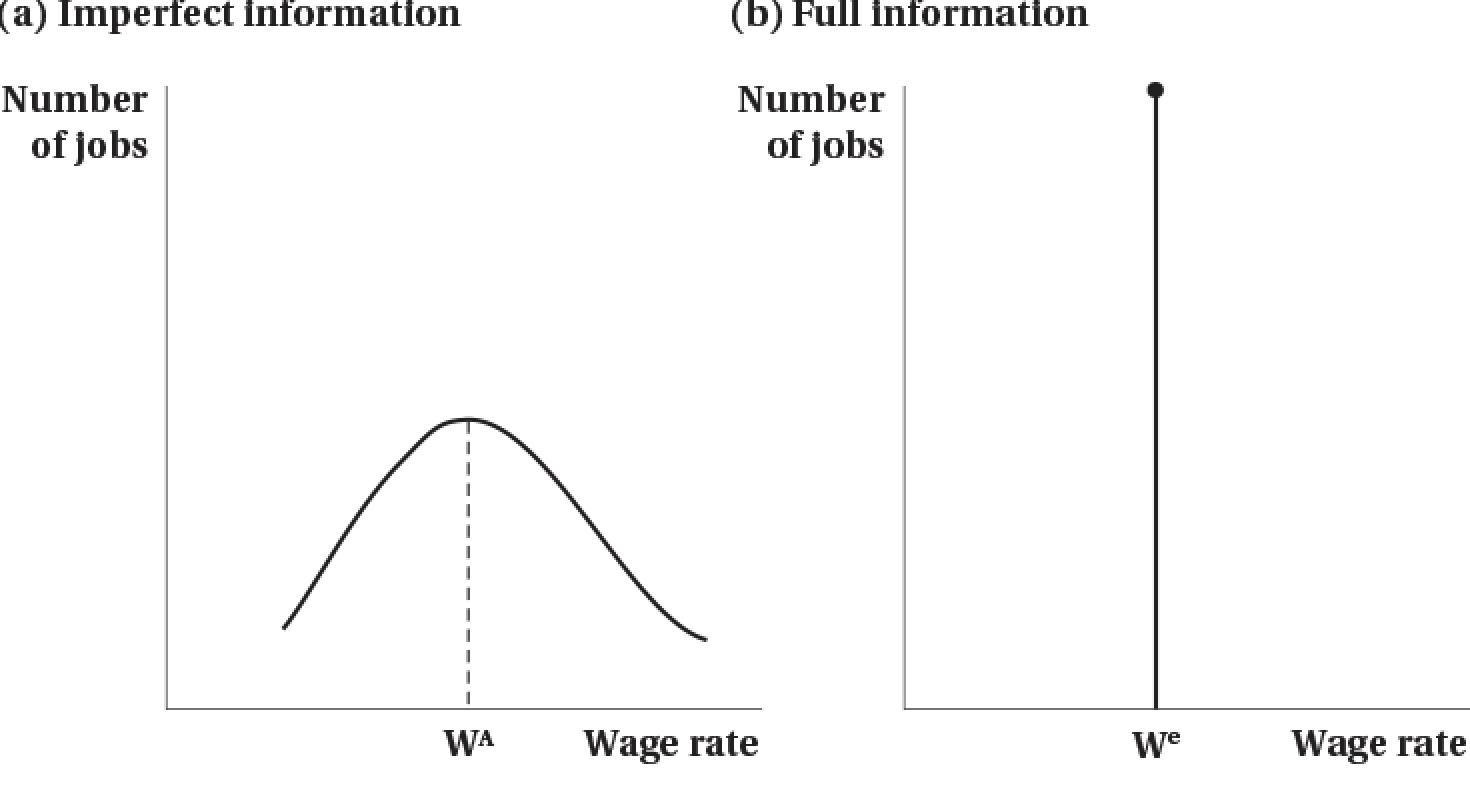
\includegraphics[scale=0.4]{wage_rate.png}
      %    \includegraphics[scale=.40]{one.pdf}
      \end{center}
  \end{figure}
\end{frame}

 \begin{frame} \frametitle{Imperfect Information in the Labour Market}
\label{imperfect info and labour market}

\textbf{Example:}

\textbf{Job Search and the Reservation Wage}\\

Julia just graduated from college and is looking for a first job.\\

There are three types of jobs: \\
\begin{itemize}
\item[]
\item The best jobs pay $\$ 2400$ a month
\item[]
\item "Not as good" jobs pay $\$ 2200$ a month
\item[]
\item The worst type of job pays $\$ 2000$ a month
\item[]
\item The probability of each type of job offered is one-third

\end{itemize}
 \end{frame}


 \begin{frame} \frametitle{Imperfect Information in the Labour Market}
\label{imperfect info and labour market}

Julia must now decide what to do once she gets an offer
\begin{itemize}
\item[]
\item The expected value of a future offer is $\$ 2200$ a month (average of $\$ 2000$,  $\$ 2200$ , and $\$ 2400$ a month)
\item[]
\item She won't accept a job offer unless it pays at least $\$ 2200$ a month
\item[]
\item $2/3$ is the hazard rate
\end{itemize}
 \end{frame}


 \begin{frame} \frametitle{Imperfect Information in the Labour Market}
\label{imperfect info and labour market}

\textbf{Factors Determining Optimal Search}
\begin{itemize}
\item[]
\item Expected benefit of job search
\item Expected duration of a job
\item Age: younger workers' unemployment duration is lower
\item Internet accessibility
\item Number of employers with available job vacancies
\item Rate at which employers offer jobs
\item Value of leisure
\item Social and labour market policies
\item Employment insurance
\item Pensions

\end{itemize}
 \end{frame}

 \begin{frame} \frametitle{Reference}
\label{Reference}

Labour Market Economics, 9th edition, by Dwayne Benjamin, Morley Gunderson, Thomas Lemieux, Craig Riddell, Tammy Schirle, 2021, McGraw-Hill Ryerson.
 \end{frame}



 \begin{frame} \frametitle{Appendix: Basic Income-Leisure Model}
\label{Appendix}

The choice of hours worked given opportunities and value of non-market time
\begin{itemize}
\item Preferences and Constraints
\item Individuals choose the feasible outcomes which yield the highest level of satisfaction
\end{itemize}

\textbf{Preferences}\\

Two "goods"
\begin{itemize}
\item Consumption
\item Leisure
\end{itemize}

Represented by indifference curves\\

\textit{	(A person is indifferent between various combinations of consumption and leisure on an indifference curve)}
 \end{frame}
 
 
 \begin{frame} \frametitle{Appendix: Basic Income-Leisure Model}
\textbf{Preferences}\\
\begin{itemize}


 \item We assume that consumers have well-defined preferences over all the conceivable combinations of consumption and leisure
 \item[]
  \item This implies that all combinations lie on some indifference curve
   \item[]
  \item Consumer preferences can then be represented by an indifference curve
   \item[]
  \item Indifference curves plot combinations of consumption and leisure that yield the consumer equal levels of utility
   \item[]
  \item The absolute value of the slope of an indifference curve gives the marginal rate of substitution (MRS); that is, the amount of leisure the consumer is willing to accept in exchange for giving up some consumption
\end{itemize}
 \end{frame}


 \begin{frame} \frametitle{Appendix: Basic Income-Leisure Model}
\textbf{Constraint}\\
\begin{itemize}


 \item  Constraints are determined by the economic properties of the market, which, in turn, transform consumption-leisure to income-leisure by setting the price of consumption
 \item[]
  \item The income and leisure combinations from which the consumer can choose with a potential income constraint
   \item[]
  \item This allows a transformation of our model from representing consumption-leisure tradeoffs to income-leisure tradeoffs.
   \item[]
  \item Alternative phrases used for the potential income constraint include budget constraint, income constraint, and full-income constraint
  
\end{itemize}
 \end{frame}
 

 \begin{frame} \frametitle{Appendix: Basic Income-Leisure Model}
\textbf{The Consumer's Optimum}\\

\begin{itemize}
\item Optimal amount of income and leisure
\item[]
 \end{itemize}
 
\textbf{Utility-maximizing equilibrium}\\
\begin{itemize}
 \item  Highest indifference curve given the income constraint
 \item[]
 \end{itemize}
 
\textbf{Compare MRS with the Market Wage Rate}

 \begin{itemize}
  \item MRS: measures the willingness to exchange leisure for consumption (or income)
 
  \item Market Wage Rate: measures the ability to exchange leisure for income
\end{itemize}
 \end{frame}





 \begin{frame} \frametitle{Appendix: Basic Income-Leisure Model}
\textbf{Change in Wage Rate on Hours of Work}\\


Two effects:
\begin{enumerate}
\item\textbf{ Income effect} The worker has more income to buy more goods including leisure (reduces work hours)
\item[]
\item \textbf{Substitution effect} Individual may work more because the returns are greater substituting away from leisure
\end{enumerate}

 \end{frame}








\end{document}
